\chapter{绪论}
\enchapter{Introduction}
\label{chap:intro}

\section{研究背景及意义}
\ensection{Research Background and Motivation}

碳纳米管（Carbon Nanotube, CNT）因其独特的准一维结构以及优异的电学、热学和力学性能，已成为纳米材料研究中的重要对象。由大量取向较一致、排列较致密的碳纳米管构成的碳纳米管阵列，不仅保留了单根 CNT 的本征优势，还因其阵列化结构更易在宏观尺度上实现集成和利用，因此在储能器件、热界面材料、场发射器件及高性能复合材料等方向表现出广阔的应用前景\cite{Hata2004,Szabo2017,Gao2023}。随着先进制造、微纳器件与高性能结构功能材料的发展，围绕 CNT 阵列开展可控生长、快速表征与规律挖掘，已经成为材料科学与智能分析交叉领域的重要研究问题。

然而，与其应用价值相比，CNT 阵列的制备与分析过程长期面临较高复杂性。当前主流制备方法之一的化学气相沉积法（Chemical Vapor Deposition, CVD）虽然具有工艺成熟、适用范围广和可扩展性较强等优点，但阵列生长结果往往同时受到温度、气体流量、碳源配比、催化剂状态、生长时间和反应压力等多种因素影响，不同参数之间还存在明显耦合\cite{Szabo2017,Bulyarskiy2020}。在这种条件下，阵列的高度、密度、取向度以及弯曲相关特征等关键形貌并不总能在相近条件下保持稳定一致。传统依赖人工经验与反复试验的研究模式虽然能够积累局部经验，但成本较高、周期较长，也难以从分散结果中沉淀出稳定、可迁移的工艺规律\cite{Gao2023}。

从表征环节来看，扫描电子显微镜（Scanning Electron Microscopy, SEM）图像是研究 CNT 阵列形貌的重要依据。针对取向、覆盖密度和局部排列状态等指标，已有研究尝试利用图像处理、傅里叶变换及自动量化方法开展定量表征\cite{Brandley2018,Imtiaz2023,Yadav2024}，但 CNT 阵列 SEM 图像通常存在边界模糊、局部交叠、遮挡、尺度不均一以及图像质量差异等问题，使得曲率、波曲度和迂曲度等弯曲相关特征的自动提取仍具有较大难度\cite{Jackman2013}。对材料研究而言，这类弯曲相关特征不仅反映阵列局部弯曲程度和形貌演化趋势，也与阵列形成过程、结构状态及潜在功能表现密切相关\cite{Wang2019DynamicCurvature,Ginga2013Waviness,Xu2012AlignmentControl,Futaba2016SweetSpot,Hajilounezhad2021}。因此，如何将依赖目视判断的图像观察转化为面向科研分析场景的关键形貌量化表征，仍是提高 CNT 阵列研究效率与一致性的现实需求。

近年来，机器学习、知识图谱与大语言模型逐步进入材料研究。一方面，机器学习方法能够从实验数据中学习工艺参数与材料结构、形貌和性能之间的对应关系，帮助研究者在小样本、高成本实验条件下缩小搜索空间并提升分析效率\cite{Hajilounezhad2021,Lookman2019}。另一方面，材料文本抽取、材料知识图谱以及领域大语言模型的发展，也使分散在文献、实验记录和工艺参数表中的信息可以被重新组织并用于后续分析\cite{Venugopal2024,Choi2024,Jiang2025,Statt2023}。与此同时，已有研究也表明，在真实材料研发场景中，通用大语言模型仍易受到领域知识覆盖不足、事实约束较弱和结果难以追溯等问题的影响；相较之下，检索增强方法在知识更新与结果溯源方面更具优势\cite{Miret2025,Mostafa2024,Soudani2024}。对于 CNT 阵列这类条件依赖强、机理复杂的研究对象而言，仅依赖通用模型仍不足以直接支撑具体科研分析任务。

综合来看，当前 CNT 阵列研究中仍存在一个更核心的问题，即工艺参数、关键形貌与生长机理三类信息长期分散在实验记录、SEM 图像及其分析结果和文献描述中，尚未形成可直接用于科研分析的稳定链条。由此带来的直接后果是，一方面关键形貌难以稳定量化，另一方面工艺—形貌关系即使能够建立，也往往缺少机理证据支撑与结果追溯能力。基于此，本文以 CNT 阵列为研究对象，以工艺—形貌关系分析为核心任务，以知识增强为支撑手段，围绕分散知识组织、关键形貌自动化表征以及工艺—形貌关系建模与解释三个层面展开研究，旨在贯通工艺参数、关键形貌与生长机理之间的分析链路，为后续工艺分析和实验判断提供更稳定、可追溯的依据。

\section{国内外研究现状}
\ensection{Research Status at Home and Abroad}

\subsection{碳纳米管阵列制备与工艺调控研究现状}
\ensubsection{Research Status on CNT Array Growth and Control}

碳纳米管阵列的制备与工艺调控研究，主要关注阵列在何种条件下实现稳定生长，以及不同工艺因素如何影响阵列的结构形貌与生长持续性。围绕这一问题，国内外学者已开展了较为系统的研究。国外早期工作通过水辅助化学气相沉积等方法显著提高了碳纳米管阵列的生长效率与纯度，为垂直排列碳纳米管阵列的进一步发展奠定了基础\cite{Hata2004}。在此基础上，相关研究逐步由单一工艺条件考察转向多参数协同调控，温度、碳源、反应气氛、催化剂层厚度和反应时间等因素对阵列高度、排列状态和生长稳定性的共同影响成为研究重点\cite{Szabo2017,Bulyarskiy2020}。近年来，相关综述又从生长机理与动力学角度总结了垂直排列碳纳米管阵列的影响因素、长度提升策略及其演化规律，为理解工艺参数与形貌变化之间的关系提供了较完整的分析框架\cite{Liu2021EcoMat}。国内研究近年来也围绕垂直排列 CNT 的可控制备与结构优化开展了持续探索，并开始尝试将文献挖掘、高通量实验和机器学习等方法结合起来，用于生长参数分析与阵列质量优化，体现出该方向由经验试错逐步向数据驱动分析发展的趋势\cite{Gao2023}。

总体来看，现有研究已经积累了较丰富的工艺调控经验，并为后续分析提供了重要基础。然而，从本文关注的问题出发，现有成果仍主要分散在具体实验体系、参数组合和文献结论之中。对于后续工艺—形貌关系分析而言，更关键的问题不在于单点实验结论不足，而在于尚缺少一种能够同时组织工艺条件、生长现象和机理解释的统一表达方式，因而难以将分散的工艺调控知识进一步转化为可组织、可调用和可分析的结构化依据。

\subsection{材料知识组织与知识增强分析研究现状}
\ensubsection{Research Status on Knowledge-Enhanced Materials Analysis}

材料知识组织与知识增强分析研究主要致力于将分散在学术文献、实验记录和结构化数据表中的信息整理为可检索、可调用并能够服务科研分析的知识。近年来，随着自然语言处理、知识图谱和大语言模型技术的发展，材料信息处理逐步形成了新的研究范式。已有研究构建了可自动生成的材料知识图谱，讨论了大语言模型在材料语言处理任务中的应用潜力，并系统梳理了自然语言处理和大语言模型在材料发现中的应用进展\cite{Venugopal2024,Choi2024,Jiang2025}。与此同时，也有研究指出，材料知识并不仅存在于高层概念描述之中，还广泛体现于样品来源、实验步骤、测试数据和元数据之间的层级关联，这使得知识图谱在承载科研分析所需上下文关系方面具有独特优势\cite{Statt2023}。国内相关研究近年来也开始关注材料知识图谱与大语言模型结合的问题，尝试利用大语言模型从材料文献中抽取结构化关系，并进一步构建面向特定材料体系的知识图谱与问答框架\cite{Bai2025}。此外，大语言模型与检索增强方法在材料发现、知识调用和辅助分析中的应用潜力，也已得到初步验证\cite{Miret2025,Mostafa2024}。

尽管如此，现有研究更多聚焦于知识抽取、关系组织和问答支撑等一般性任务，检索增强方法也主要服务于通用知识调用与辅助分析。对本文而言，更关键的是建立一种能够统一组织文献、实验记录、工艺参数表和图像分析结果的知识表示与证据组织机制，为后续检索、结果追溯和分析解释提供支撑。也就是说，当前仍缺少一种能够直接服务 CNT 阵列科研分析场景的知识表示与检索机制。

\subsection{CNT 阵列 SEM 图像分析与形貌表征研究现状}
\ensubsection{Research Status on SEM-Based Morphology Characterization}

CNT 阵列 SEM 图像分析与形貌表征研究，主要关注如何将依赖经验判断的图像观察结果转化为可比较、可分析的结构化指标。围绕这一问题，已有研究围绕取向度、排列状态和局部结构特征开展了较多探索。已有研究利用快速傅里叶变换对扫描电子显微镜图像中的碳纳米管取向进行映射，也有研究提出了基于图像处理的配向度估计方法和垂直排列程度定量评价思路\cite{Brandley2018,Imtiaz2023,Yadav2024}。与此同时，关于碳纳米管扫描电子显微镜成像机理及其本征尺寸恢复问题的讨论，也为理解 CNT 图像中的结构信息提供了基础\cite{Jackman2013}。相关研究还表明，CNT 阵列形貌可在较规整的森林状结构与更明显的起伏波曲结构之间发生变化，这说明弯曲相关特征及排列均匀性本身就是值得重点关注的关键形貌信息\cite{Zhang2009Morphology}。

从现有研究进展来看，CNT 图像中的部分结构信息已经能够被转化为定量指标，自动化分析也具备了一定基础。同时，也已有研究尝试利用语义分割方法稳定提取 CNT 前景，并通过单纤维分离与连续追踪进一步恢复个体级结构，说明复杂细长网络中的前景提取已具备一定可行性。然而，对本文后续工艺—形貌关系分析而言，更关键的并不是继续增加图像指标种类，而是获得稳定、可比较的关键形貌标签，尤其是围绕曲率、波曲度和迂曲度等弯曲相关特征建立可靠的样品级表征方式。现有方法在这一方面仍存在不足，一是弯曲相关特征提取对图像质量、交叉黏连和局部遮挡较为敏感，二是对局部几何扰动与整体结构均匀性共同变化的表征能力仍然有限。因此，如何面向 CNT 阵列建立稳定的样品级关键形貌表征流程，仍是当前研究中的重要问题。

\begin{figure}[htbp]
    \centering
    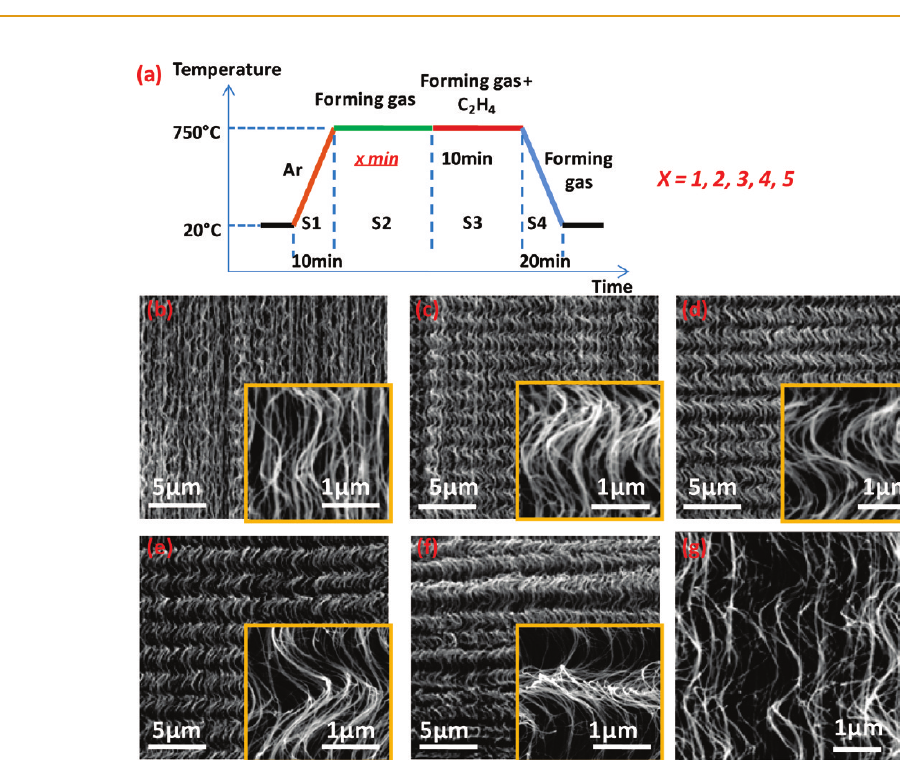
\includegraphics[width=0.92\textwidth]{figures/intro_cnt_morph_original.png}
    \caption{起伏 CNT 阵列的生长条件与典型 SEM 形貌（引自文献\cite{Zhang2009Morphology}，经裁剪）}
    \label{fig:intro_cnt_morph}
\end{figure}

\subsection{工艺参数分析、形貌关系分析与实验优化研究现状}
\ensubsection{Research Status on Morphology Relation Modeling and Experimental Optimization}

工艺参数分析、形貌关系分析与实验优化研究，主要关注如何利用已有数据刻画工艺条件与阵列形貌之间的关系，并进一步为实验设计与参数选择提供依据。围绕这一问题，数据驱动方法已在材料科学中得到广泛关注。已有研究利用模拟图像、深度学习和数据驱动方法对 CNT 阵列的结构属性与力学行为进行预测，表明工艺、结构和性能之间的映射关系在一定条件下能够通过模型学习加以近似刻画\cite{Hajilounezhad2021}。与此同时，主动学习、贝叶斯优化和闭环实验优化等方法也已被系统总结，并被广泛用于应对样本有限、实验成本高和参数空间较大的问题\cite{Lookman2019}。在 CNT 研究中，已有工作给出了利用贝叶斯优化提升生长速率的闭环实验案例\cite{Chang2020}；国内研究也开始将文献挖掘、机器学习与高通量制备相结合，用于关键生长参数分析及阵列高度、质量优化\cite{Gao2023}。进一步地，机器学习模型、自动化实验与机器人 CVD 平台的结合，也说明该方向正由单点分析逐步走向更紧密的人机协同研究模式\cite{Li2025Matter}。

总体来看，数据驱动方法已经能够在 CNT 阵列研究中用于参数分析与实验优化。然而，从本文的研究目标出发，若关键形貌标签本身缺乏稳定性，或分析结果缺少与领域机理相衔接的证据支撑，则模型输出即使在数值上具有一定效果，也难以真正转化为可靠的科研判断依据。因此，对本文而言，更合理的研究路径并不是直接追求实验优化闭环，而是先建立稳定的关键形貌表征方式，再在此基础上形成具有知识证据支撑的工艺—形貌关系分析框架。

综上，围绕 CNT 阵列的制备调控、材料知识组织、SEM 图像表征以及数据驱动分析，国内外研究都已形成一定基础。在工艺层面，已有较多关于阵列生长调控的实验认识；在知识层面，知识图谱与检索增强为多源信息组织提供了方法基础；在表征层面，CNT 图像中的部分结构信息已能够转化为定量指标；在分析层面，数据驱动方法也已能够用于参数分析与实验优化。尽管如此，从服务科研分析任务的角度看，现有工作仍未形成一条贯通工艺参数、关键形貌与生长机理的完整分析路径。前端缺少面向多源科研材料的统一知识组织方式，中间缺少稳定、可比较的关键形貌标签，后端缺少能够将工艺—形貌分析结果与机理证据衔接起来的解释机制。正因为上述三个环节尚未真正打通，工艺参数、关键形貌与生长机理之间的关系仍未得到有效连接。本文即围绕这一问题展开研究，并在后文分别从知识建模与检索增强、关键形貌自动化表征以及知识增强支持下的工艺—形貌关系分析三个方面加以展开。

\section{本文研究内容与技术路线}
\ensection{Research Content and Technical Route}

针对上述问题，本文以 CNT 阵列为研究对象，以工艺—形貌关系分析为核心任务，以知识增强为贯穿支撑手段，围绕知识组织、关键形貌表征、关系建模和结果解释展开研究，目标是构建一条贯通多源知识组织、样品级关键形貌提取、工艺—形貌关系分析与知识增强解释的分析链路。

本文的研究主要包括三个部分。第一部分研究面向碳纳米管阵列的多源知识建模与检索增强方法，处理文献、实验记录、工艺参数和图像分析结果的统一组织问题，为工艺分析、形貌解释和结果追溯提供证据支撑。第二部分研究 CNT 阵列关键形貌自动化表征方法，围绕 SEM 图像建立样品级自动化表征流程，获取取向度、平均曲率、波曲度和迂曲度等关键形貌特征，为后续关系分析提供稳定标签。第三部分研究知识增强支持下的工艺—形貌关系分析与解释方法，在知识检索结果支持下围绕 Fe 功率、Fe 厚度和退火时间等工艺变量开展统计关系分析与预测建模，并结合知识库中的机理证据对关键变量作用及预测结果进行解释。前述方法最终通过科研辅助分析平台完成集成实现与流程验证。

本文整体遵循“知识组织—关键形貌表征—关系建模—结果解释”的技术路线。先面向文献、实验记录、工艺参数表和图像分析结果构建统一知识组织框架，通过 MSFU 表示与关系约束检索获得证据链，为后续变量筛选和机理解释提供支撑。再针对 SEM 图像建立自动化关键形貌表征流程，获取取向度、平均曲率、波曲度和迂曲度等样品级结构化特征，并结合知识检索结果识别工艺—形貌关系线索，为关系建模提供稳定标签。随后，在前述形貌标签与知识线索支持下，围绕 Fe 功率、Fe 厚度和退火时间等工艺变量开展统计关系分析与预测建模。最后，将知识检索结果与样品级分析结果结合起来，对关键变量作用及预测结果进行解释，并通过科研辅助平台完成方法集成与流程验证。技术路线如图~\ref{fig:1_1} 所示。

\begin{figure}[htbp]
    \centering
    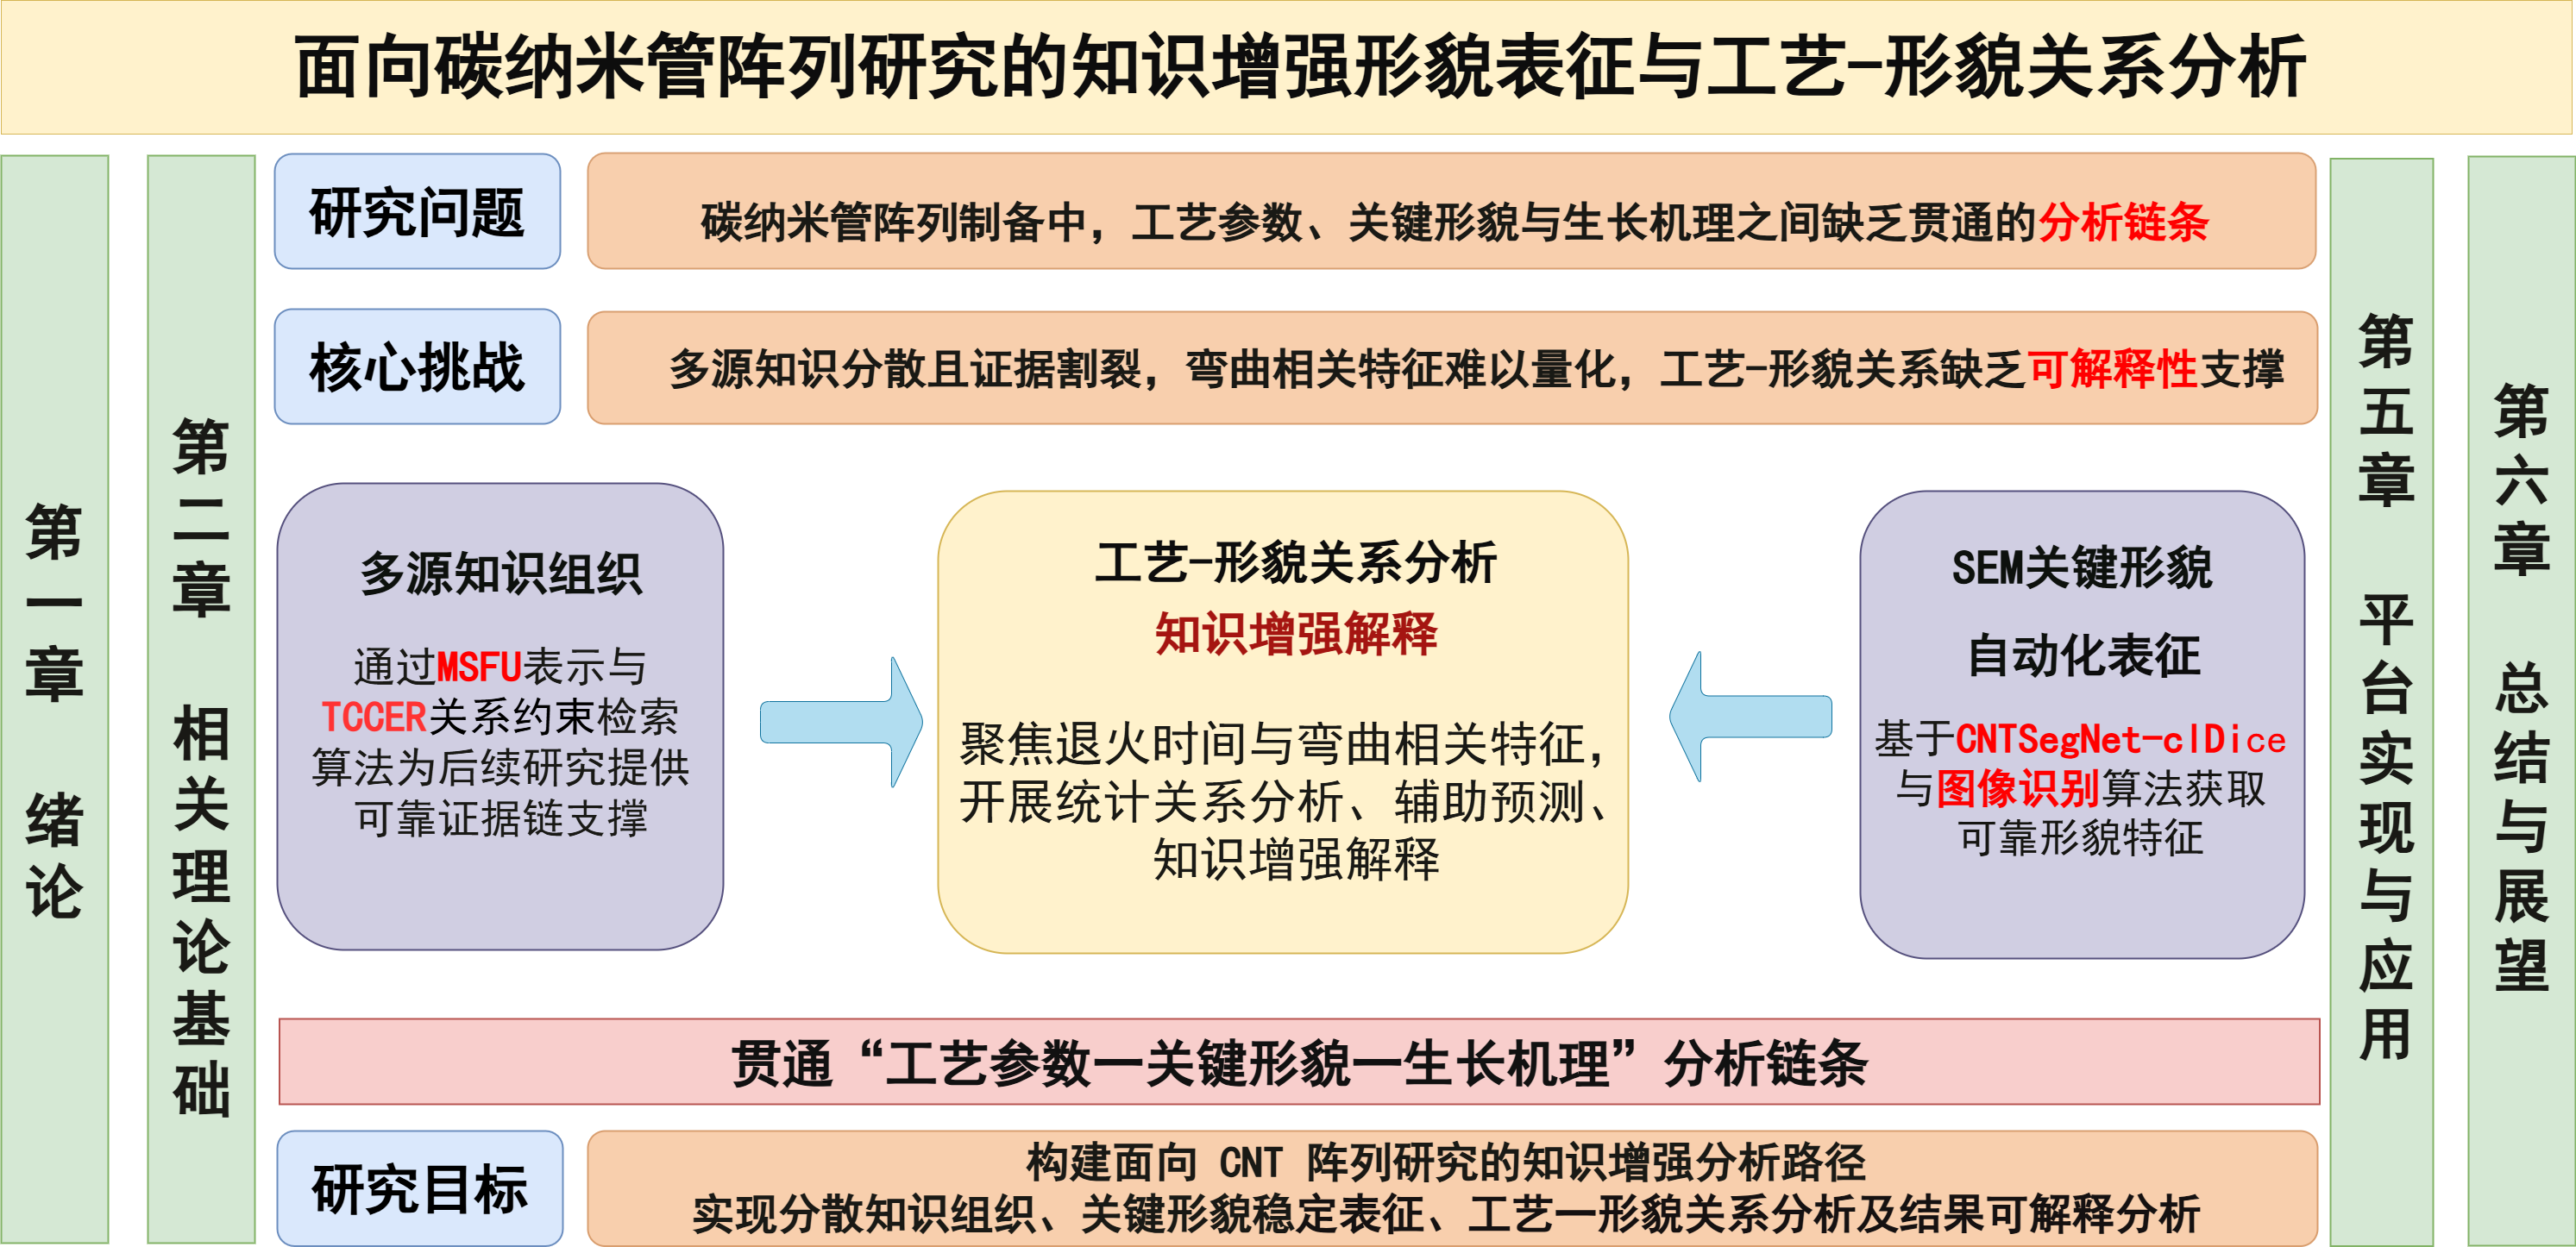
\includegraphics[width=0.98\textwidth]{figures/fig1-1-main-framework.png}
    \caption{本文技术路线图}
    \label{fig:1_1}
\end{figure}

本文的工作主要有三点特点。其一，面向 CNT 阵列科研分析任务，提出以最小语义事实单元为核心的多源知识组织方式，并构建关系约束检索方法，使工艺参数、关键形貌、生长机理与文献证据能够在同一框架下组织和调用。其二，提出服务于工艺—形貌关系分析的关键形貌自动化表征方法，围绕曲率、波曲度和迂曲度等弯曲相关特征构建样品级结构化表示，使依赖经验判断的弯曲形貌转化为可比较、可分析的结构化特征。其三，提出面向碳纳米管阵列工艺—形貌分析的知识增强解释框架，将知识库中识别出的关系线索与样品级统计分析结果结合起来，用于说明关键变量作用及其可能机制。

本文共分为六章。第一章为绪论，介绍研究背景、国内外研究现状，并说明本文的研究内容与技术路线。第二章介绍本文研究所涉及的相关理论与关键技术，包括知识组织方法、CVD 工艺机理、图像处理方法及工艺关系分析方法。第三章研究面向 CNT 阵列科研任务的知识建模与检索增强方法，解决多源知识分散、证据难以成链的问题。第四章开展 CNT 阵列 SEM 图像关键形貌自动化表征与工艺—形貌关系分析，讨论特征提取方法、参数关系分析及知识增强解释。第五章对前述方法进行系统集成，设计并实现面向 CNT 阵列研究的科研辅助分析平台，并对平台功能进行测试。第六章对全文进行总结，归纳研究成果与不足，并对后续研究方向进行展望。

围绕上述问题，本文形成了“知识组织—关键形貌表征—关系分析—结果解释”的总体技术路线。其中，第 3 章重点解决多源知识组织与证据链检索问题，第 4 章重点解决关键形貌表征与工艺—形貌关系分析问题，第 5 章对前述方法进行系统集成与验证。
